\chapter{\texorpdfstring{The Coherence Functions $g^{(1)}$, $g^{(2)}$ and the Siegert Relation}{The Coherence Functions g1, g2 and the Siegert Relation}}
\label{chap:e08}

\begin{chapteropening}
By now, what the telescope hands us is no longer "a blob of brightness" but the \textbf{event list} introduced in Chapter \ref{chap:e07}: a string of time-stamped "clicks." The question we now ask is no longer "how bright is it on average," but something far more subtle: \emph{do these clicks bear any relationship to one another?} If the photons in two detectors, in two time gates, arrive merely at random and independently, then their occasional simultaneous firing is pure coincidence; but if they fire together \emph{more often than chance}, or \emph{less often than chance}, then the event list hides the fingerprint of the light field's statistics. This chapter teaches you a language for translating "the event list" into "the statistics of the light field": first-order coherence \(g^{(1)}\) measures the phase memory of the electric field, while second-order coherence \(g^{(2)}\) measures the tendency of photons to arrive in pairs. What connects the two is the climax of this chapter: the Siegert relation. It reveals something close to magic: by counting nothing but the "degree of synchrony" of intensity fluctuations, you can read off the squared modulus of the field's degree of coherence. This is precisely what underwrites all of the intensity interferometry and imaging that follows.
\end{chapteropening}

\section{Why Give "Correlation" a Function of Its Own}
\label{sec:e08-why-correlation}

Let us first catch the conclusions of the previous stage. Chapter \ref{chap:e02} told us that light "remembers" its own phase only within a very short coherence time \(\tau_c\); in the broadband visible, \(\tau_c\) is as short as picoseconds, while detectors are as slow as hundreds of picoseconds or more, so a single time gate averages over hundreds or thousands of mutually incoherent wave trains. Chapter \ref{chap:e06} then told us that different states of light (coherent, thermal, number states) can share exactly the same mean brightness yet differ enormously in their photon-number \emph{fluctuations}. Put these two facts together and a natural thought arises: \emph{since the total intensity of a single exposure has erased so much information, could we stop looking at the "total" and instead look at the "echo between two detections"?}

This is exactly where the coherence function comes into its own. Its idea is extremely plain, and it descends directly from the autocorrelation function of Chapter \ref{chap:e02}: take the light field (or the photon stream) and compare it with "a copy of itself delayed by \(\tau\)," and see how alike they still are. The only difference lies in \emph{what} is compared:

\begin{itemize}
  \item If we compare the \textbf{amplitude and phase of the electric field}, we obtain first-order coherence \(g^{(1)}(\tau)\): it answers "how much phase does the field still remember after a delay \(\tau\)?" Amplitude interferometry (Chapter \ref{chap:e09}) uses precisely this.
  \item If we compare the \textbf{intensity (photon arrivals)}, we obtain second-order coherence \(g^{(2)}(\tau)\): it answers "are two detection events more likely to appear in pairs than the random case?" Hanbury Brown--Twiss (HBT) intensity interferometry uses precisely this \citep{1956Natur.177...27B}.
\end{itemize}

The reason we write "correlation" as \emph{a function of the delay \(\tau\)}, rather than a single number, is that the strength of the echo varies with delay: the echo is strongest at very small delay, and once the delay is stretched beyond the coherence time, the two detections lose all "contact." The \emph{height} and \emph{width} of this echo-versus-\(\tau\) decay curve encode, respectively, the kind of light (thermal or laser) and its spectral width (coherence time). This chapter will lay out both of these curves one by one, and then join them with a single bridge: the Siegert relation.

\section{First-Order Coherence: How Much Phase Does the Field Remember Across \texorpdfstring{$\tau$}{tau}}
\label{sec:e08-g1}

Let us begin with the easiest to picture, the first order. In Chapter \ref{chap:e05} we wrote the positive-frequency electric field on the detector surface as the operator \(\hat E^{(+)}(t)\) (which contains only the annihilation operator \(\hat a\), whose action is to "remove one photon"), and its Hermitian conjugate \(\hat E^{(-)}(t)\) (which contains only the creation operator \(\hat a^\dagger\)) is the negative-frequency part. The first-order coherence function is defined by "multiplying the fields at two instants and averaging":

\begin{equation}
  G^{(1)}(t_1,t_2)=\big\langle \hat E^{(-)}(t_1)\,\hat E^{(+)}(t_2)\big\rangle,
  \qquad
  g^{(1)}(\tau)=\frac{G^{(1)}(t,t+\tau)}{G^{(1)}(t,t)} .
  \label{eq:e08-g1}
\end{equation}
\begin{formulaexplain}
\(G^{(1)}\) is the first-order field correlation; \(\hat E^{(+)},\hat E^{(-)}\) are the positive- and negative-frequency field operators; \(\langle\cdot\rangle\) is the expectation over the quantum state; \(g^{(1)}\) is the normalized version obtained by dividing by the zero-delay value; \(\tau=t_2-t_1\) is the delay. It measures how much phase memory the field still retains across a delay \(\tau\).
\end{formulaexplain}

Let us pin down every symbol. \(G^{(1)}(t,t)=\langle\hat E^{(-)}(t)\hat E^{(+)}(t)\rangle\) is just the mean intensity at time \(t\) (a positive real number, carrying the dimensions of intensity), so after normalization \(g^{(1)}\) is a dimensionless complex number. If the light field is \emph{statistically stationary} (its statistical properties do not drift with absolute time, the normal condition for a stable source), the correlation depends only on the delay \(\tau\) and not on the starting point \(t\), so \(g^{(1)}\) becomes a function of \(\tau\) alone. Its modulus \(|g^{(1)}(\tau)|\) lies between \([0,1]\), and its physical meaning can be captured in a single sentence:

\begin{itemize}
  \item \(|g^{(1)}(\tau)|\to1\): the field after a delay \(\tau\) is still in step with the original field, its phase predictable: \textbf{coherent}. Superpose it with its pre-delay self and it will draw out sharp interference fringes.
  \item \(|g^{(1)}(\tau)|\to0\): the field has completely forgotten the phase it held \(\tau\) ago: \textbf{amnesia}. Superposition now gives a smeared-out, fringe-free brightness.
\end{itemize}

This is precisely the "field version" of the autocorrelation function \(\Gamma(\tau)\) of Chapter \ref{chap:e02}: the width over which \(g^{(1)}(\tau)\) decays from its peak of 1 down to 0 is the coherence time \(\tau_c\). And \(\tau_c\) is set by the spectral width; recall the two formulas of Chapter \ref{chap:e02}:

\begin{equation}
  \Delta\nu\simeq\frac{c\,\Delta\lambda}{\lambda^2},
  \qquad
  \tau_c\simeq\frac{1}{\Delta\nu}\simeq\frac{\lambda^2}{c\,\Delta\lambda}.
  \label{eq:e08-tauc}
\end{equation}
\begin{formulaexplain}
\(\Delta\nu\) is the frequency bandwidth (Hz), \(\Delta\lambda\) is the wavelength bandwidth, \(\lambda\) is the central wavelength, \(c\) is the speed of light, and \(\tau_c\) is the coherence time (s). It converts "how narrow the filter is" directly into "how long the field's phase memory lasts."
\end{formulaexplain}

Let us plug in real numbers to feel the magnitude. Take a "very narrow" filter: central wavelength \(\lambda=780\,{\rm nm}\), bandwidth \(\Delta\lambda=1\,{\rm nm}\). First compute the frequency bandwidth (in CGS, \(c=3\times10^{10}\,{\rm cm\,s^{-1}}\), \(\lambda=7.8\times10^{-5}\,{\rm cm}\), \(\Delta\lambda=10^{-7}\,{\rm cm}\)):
\[
  \Delta\nu\simeq\frac{(3\times10^{10})(10^{-7})}{(7.8\times10^{-5})^2}
  =\frac{3\times10^{3}}{6.1\times10^{-9}}
  \approx4.9\times10^{11}\,{\rm Hz},
\]
so
\[
  \tau_c\simeq\frac{1}{4.9\times10^{11}\,{\rm Hz}}\approx2\times10^{-12}\,{\rm s}=2\,{\rm ps}.
\]
That is to say, even through a 1-nanometer narrowband filter, the electric field of a star's thermal light remembers its own phase for only about 2 picoseconds before turning the page. This 2 ps will reappear again and again in this chapter, and it will directly set how narrow the later intensity-correlation peak is, and by how many factors it is diluted.

\section{Second-Order Coherence: Do Photons Like to Arrive in Pairs}
\label{sec:e08-g2}

Change the question from "does the field still remember the phase" to "are two detection events correlated," and we enter the second order. The definition given by the quantum theory of photodetection (Chapter \ref{chap:e07}) is the average of four field operators arranged in a particular order:

\begin{equation}
  G^{(2)}(t_1,t_2)=\big\langle
    \hat E^{(-)}(t_1)\,\hat E^{(-)}(t_2)\,\hat E^{(+)}(t_2)\,\hat E^{(+)}(t_1)
  \big\rangle,
  \qquad
  g^{(2)}(\tau)=\frac{G^{(2)}(t,t+\tau)}{G^{(1)}(t,t)\,G^{(1)}(t+\tau,t+\tau)} .
  \label{eq:e08-g2-field}
\end{equation}
\begin{formulaexplain}
\(G^{(2)}\) is the second-order field correlation; among the four operators, the two creation operators (\(\hat E^{(-)}\)) are all placed on the left and the two annihilation operators (\(\hat E^{(+)}\)) are all placed on the right: this is called \textbf{normal ordering}; as for the inner/outer nesting, it is paired by time (the \(t_1\) pair on the outermost layer, the \(t_2\) pair on the inner layer), guaranteeing the time order "absorb first at \(t_1\), then absorb at \(t_2\)." The denominator is the product of the mean intensities at the two instants; \(g^{(2)}\) is the normalized result. It measures whether photons tend to arrive in pairs.
\end{formulaexplain}

This formula deserves to be read slowly, term by term, because each term corresponds to something countable in the event list.

\textbf{Why this strange operator ordering?} Chapter \ref{chap:e07} explained that what a detector "counts" is the event of \emph{absorbing} a photon, and each absorption uses up one annihilation operator \(\hat E^{(+)}\). To detect one photon at each of the two instants \(t_1\) and \(t_2\), we apply two annihilation operators \(\hat E^{(+)}(t_2)\hat E^{(+)}(t_1)\) in succession to the state, obtaining the state vector \(\hat E^{(+)}(t_2)\hat E^{(+)}(t_1)|\psi\rangle\); the probability of this joint detection is exactly its squared modulus \(\big|\hat E^{(+)}(t_2)\hat E^{(+)}(t_1)|\psi\rangle\big|^2\), which upon expansion moves the two creation operators, unchanged, to the left. Thus the creation operators all sit on the left and the annihilation operators all on the right; this is normal ordering, and it guarantees that what we count are \emph{two distinct absorption events}, not the spurious term of a single photon pairing with itself. As for the "outer/inner" nesting in the formula, it comes purely from time pairing: the \(t_1\) pair (one creation, one annihilation) sits on the outermost layer, the \(t_2\) pair on the inner layer, locking in the temporal order "absorb first at \(t_1\), then absorb at \(t_2\)." This is a different matter from "creation on the left, annihilation on the right"; do not conflate them. This point was already foreshadowed in Chapter \ref{chap:e07}'s factorial moment \(\langle N(N-1)\rangle\): what the detector admits are ordered pairs made of distinct photons.

\textbf{What is the denominator?} The denominator \(G^{(1)}(t,t)\,G^{(1)}(t+\tau,t+\tau)=\langle I(t)\rangle\langle I(t+\tau)\rangle\) is the baseline of "how many accidental coincidences there should be if the two detections were completely independent." In other words, if the photons at the two instants are entirely uncorrelated, each arriving at random at its own mean rate, then the joint rate of their happening to be detected together is just the product of the two mean rates.

\textbf{What is the numerator?} The numerator is the true \emph{joint} detection intensity. Divide it by the "accidental-coincidence baseline of the independent case" and \(g^{(2)}\) becomes a dimensionless \emph{relative excess}:

\begin{itemize}
  \item \(g^{(2)}(\tau)=1\): the true coincidence exactly equals the random baseline, and photon arrivals are mutually independent. The ideal laser (coherent state, Chapter \ref{chap:e06}) is just like this: it gives Poisson counts, \(g^{(2)}=1\).
  \item \(g^{(2)}(0)>1\): near zero delay there are \emph{more} photon pairs than random, and photons like to cluster, called \textbf{bunching}. Ideal single-mode thermal light gives the beautiful value \(g^{(2)}(0)=2\).
  \item \(g^{(2)}(0)<1\): the zero-delay coincidence is \emph{suppressed}, and photons avoid one another, called \textbf{antibunching}. This cannot be explained by any positive-definite classical intensity fluctuation, and is the standard \emph{nonclassical} signature of single-photon sources and resonance fluorescence \citep{1977PhRvL..39..691K}.
\end{itemize}

Why is ideal single-mode thermal light exactly 2? The physical picture was already laid down in Chapter \ref{chap:e06}: the electric field of thermal light is the superposition of many small contributions with random phases, so the instantaneous intensity forms a random speckle of bright and dark patches; within a "bright patch" the detector is more likely to record several photons in succession, so coincidences rise near zero delay. And the specific number 2 is precisely the direct corollary of the next section's Siegert relation evaluated at \(\tau=0\); keep this suspense in mind for now.

In engineering estimates people often write the same thing in terms of continuous intensity:

\begin{equation}
  g^{(2)}(\tau)=\frac{\big\langle I(t)\,I(t+\tau)\big\rangle}{\big\langle I(t)\big\rangle^2}.
  \label{eq:e08-g2-classical}
\end{equation}
\begin{formulaexplain}
\(I(t)\) is the intensity (or the detector current or count rate proportional to it); the numerator is the joint fluctuation of the intensity at the two instants; the denominator is the square of the mean intensity (using stationarity, so the mean at the two instants is the same). This is the "classical form" of second-order coherence, convenient for estimation.
\end{formulaexplain}

This line is convenient, but it hides a \textbf{trap} that must be spelled out: which intensity is \(I(t)\), exactly? It could be the ideal \emph{instantaneous} intensity of the light field, or it could be the detector output current, the event rate recorded by the TDC, or the sampled ADC value. These two are worlds apart: the latter has already been \emph{convolved} by the detector's few-nanosecond response. If you plug into Eq.~\eqref{eq:e08-g2-classical} an \(I(t)\) that has been smeared by a 4 ns electronic response, what you get is the "post-response" \(g^{(2)}\), not the picosecond-wide correlation peak of the light field itself. Many astronomical intensity-correlation signals are not "unbunched"; rather, that peak, which should have risen to 2, has been suppressed by the finite time response, by multiple modes, and by background light down to \(10^{-3}\), \(10^{-6}\), or even smaller (Section \ref{sec:e08-telescope} will settle this account). So every time you write down Eq.~\eqref{eq:e08-g2-classical}, ask yourself one question: this \(I\), has it been convolved?

\section{The Siegert Relation: Reading the Squared Field Coherence from the Intensity Correlation}
\label{sec:e08-siegert}

Now we reach the climax of this chapter. The previous two sections each defined \(g^{(1)}\) (field phase memory) and \(g^{(2)}\) (photon pairing tendency), and they look like two entirely separate things: one about phase, one about intensity. The central miracle of the HBT experiment is this: for \textbf{Gaussian chaotic light} (that is, light such as thermal light, formed by the random superposition of a large number of independent small contributions), there exists an exact bridge between the two. Cross this bridge, and using only the measurement "count the intensity fluctuations" (something a detector can do) you can infer the field's degree of coherence, the phase information a detector "cannot see."

\paragraph{The Key Tool: the Gaussian Moment Theorem (Wick's Theorem)}
\label{sec:e08-gaussian-moment}

The pier of this bridge is a theorem from statistics, which we will first spell out on its own, never quietly substituting it in.

The electric field \(E(t)\) of thermal light is the random-phase superposition of a vast number of independent radiators (atoms, electrons). By the \textbf{central limit theorem} (the sum of a large number of independent random quantities tends toward a Gaussian distribution), the complex field \(E=E_r+iE_i\) approximately follows a \emph{zero-mean circularly symmetric complex Gaussian} distribution. The phrase "circularly symmetric" is crucial: it means the phase of the field is completely uniform over \([0,2\pi)\), from which we can deduce a property we will use immediately:

\begin{equation}
  \langle E(t_1)\,E(t_2)\rangle=0,
  \qquad\text{but}\qquad
  \langle E^*(t_1)\,E(t_2)\rangle=G^{(1)}(t_1,t_2)\neq0.
  \label{eq:e08-circular}
\end{equation}
\begin{formulaexplain}
The average of two fields multiplied together (neither starred) is zero, because their total phase is random and the positives and negatives cancel; only when one is starred and one is not does the phase cancel and a nonzero correlation survive. This is the defining property of a circularly symmetric Gaussian field.
\end{formulaexplain}

For such a field, the \textbf{Gaussian moment theorem} (called Isserlis's theorem in probability and Wick's theorem in quantum field theory) states: \emph{any higher-order moment can be decomposed into a sum of second-order moments (pairwise pairings), running over all ways of pairing}. And by Eq.~\eqref{eq:e08-circular}, only pairings of "one starred with one unstarred" are nonzero; all the rest vanish. This is all we will use: it is not an approximation, but a rigorous algebraic fact about the zero-mean circular Gaussian distribution.

\paragraph{Splitting the Fourth-Order Moment}
\label{sec:e08-factorize}

Now let us get to work. The numerator of the second-order coherence (written with classical intensity, \(I=E^*E\)) is a fourth-order moment:
\[
  \big\langle I(t)\,I(t+\tau)\big\rangle
  =\big\langle E^*(t)\,E(t)\,E^*(t+\tau)\,E(t+\tau)\big\rangle .
\]
Among the four fields, two are starred (\(E^*(t),E^*(t+\tau)\)) and two are unstarred (\(E(t),E(t+\tau)\)). By the Gaussian moment theorem, pair them two by two, keeping only the "starred with unstarred" terms. There are two legal pairings:

\emph{Pairing one}: \(E^*(t)\) with \(E(t)\), \(E^*(t+\tau)\) with \(E(t+\tau)\), each paired "in place." This gives
\[
  \langle E^*(t)E(t)\rangle\,\langle E^*(t+\tau)E(t+\tau)\rangle
  =\langle I(t)\rangle\,\langle I(t+\tau)\rangle=\langle I\rangle^2 .
\]

\emph{Pairing two}: \(E^*(t)\) with \(E(t+\tau)\), \(E^*(t+\tau)\) with \(E(t)\), a "cross" pairing. This gives
\[
  \langle E^*(t)E(t+\tau)\rangle\,\langle E^*(t+\tau)E(t)\rangle
  =G^{(1)}(\tau)\,G^{(1)}(-\tau)
  =G^{(1)}(\tau)\,\big[G^{(1)}(\tau)\big]^*
  =\big|G^{(1)}(\tau)\big|^2 .
\]
(Here we used the symmetry of a stationary field, \(G^{(1)}(-\tau)=[G^{(1)}(\tau)]^*\).) Adding the two terms:

\begin{equation}
  \big\langle I(t)\,I(t+\tau)\big\rangle=\langle I\rangle^2+\big|G^{(1)}(\tau)\big|^2 .
  \label{eq:e08-G2-factor}
\end{equation}
\begin{formulaexplain}
The left side is the measurable intensity correlation; on the right, the first term \(\langle I\rangle^2\) is the "random baseline of the independent case," and the second term \(|G^{(1)}(\tau)|^2\) is the extra fluctuation contributed by the field's degree of coherence. The fourth-order moment has thus been split into a sum of two second-order moments.
\end{formulaexplain}

Divide both sides by \(\langle I\rangle^2\), and noting that \(|g^{(1)}(\tau)|^2=|G^{(1)}(\tau)|^2/\langle I\rangle^2\), we immediately obtain the ideal form of the \textbf{Siegert relation}:
\[
  g^{(2)}(\tau)=1+\big|g^{(1)}(\tau)\big|^2 \qquad(\text{ideal single spatio-temporal-polarization mode}).
\]
At \(\tau=0\), \(|g^{(1)}(0)|=1\), so \(g^{(2)}(0)=1+1=2\). The suspense of the last section ("why is thermal light exactly 2") is now resolved: that 2 is the 1 of the random baseline, plus the 1 contributed when the field is fully coherent.

\paragraph{Installing It in a Real Telescope: the Visibility Factor \texorpdfstring{$\zeta$}{zeta}}
\label{sec:e08-zeta}

Real detection is never so ideal as "a single spatio-temporal-polarization mode." Unpolarized light mixes at least two polarizations, a broad spectrum has several frequency modes, atmospheric jitter (seeing, the phenomenon of a stellar image being blurred by turbulence) produces an image with several spatial speckles, and background light seeps in to dilute; all of these suppress that ideal 1. Bundle all these dilution factors into one \textbf{visibility factor} \(\zeta\), and the Siegert relation takes the signature form of this chapter:

\begin{equation}
  \boxed{\,g^{(2)}(\tau)=1+\zeta\,\big|g^{(1)}(\tau)\big|^2\,},
  \qquad 0<\zeta\le1 .
  \label{eq:e08-siegert}
\end{equation}
\begin{formulaexplain}
\(g^{(2)}-1\) is the excess of the intensity correlation; \(|g^{(1)}|^2\) is the squared modulus of the first-order field coherence; \(\zeta\) collects the dilution at the level of the \emph{true correlation} (mode number, polarization, background) and equals 1 for the ideal single mode. The finite time response is \emph{not} counted in \(\zeta\); it is handled separately by convolution in Section \ref{sec:e08-telescope}. This is the core bridge by which HBT reads the squared field coherence from the intensity correlation.
\end{formulaexplain}

Let us account for the sources of \(\zeta\) term by term: unpolarized thermal light already has \(M_{\rm pol}\simeq2\) polarization modes, which pulls the peak height from 2 down to 1.5 (i.e.\ \(\zeta\simeq1/2\)); multiple spatial speckles and multiple frequency modes each multiply by a further \(1/M\); and if the source photons account for fractions \(f_A,f_B\) of the total counts in the two channels (the rest being background), the correlation amplitude must be multiplied approximately by \(f_Af_B\). The product of these factors can easily push \(\zeta\) below \(10^{-3}\), which is why an astronomical HBT plot shows the decimal of \(g^{(2)}-1\), rather than the clean 1 of the textbook.

The significance of Eq.~\eqref{eq:e08-siegert} cannot be overstated: \emph{the left side is the intensity correlation that the event list can directly measure, while the \(g^{(1)}\) on the right is the field's degree of coherence}. And we have two independent routes to \(g^{(1)}\): it is the Fourier transform of the spectral line shape (the Wiener--Khinchin theorem, Chapter \ref{chap:e02}), and it is also the fringe visibility measured by an amplitude interferometer (Chapter \ref{chap:e09}). Thus the "degree of synchrony" of the intensity fluctuations is converted into the squared modulus of the field's degree of coherence.

\begin{figure}[tbp]
\centering
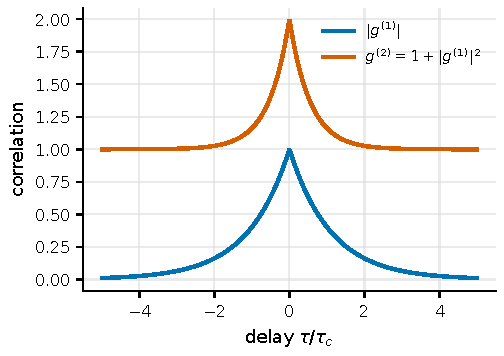
\includegraphics[width=0.86\linewidth]{figures/generated/chapter_04/ch04_siegert_relation.pdf}
\caption{The Siegert relation converts the decay of the first-order field coherence into the second-order intensity bunching peak. If \(|g^{(1)}(\tau)|\) decays with delay over the coherence time \(\tau_c\), then \(g^{(2)}(\tau)-1\) decays as \(|g^{(1)}(\tau)|^2\) and returns to the uncorrelated value 0 at large delay; the zero-delay peak height is 1 for the ideal single mode, and in real observations must be multiplied by the visibility factor \(\zeta\) (mode number, polarization, background; the finite time response is not included in \(\zeta\) but handled separately by convolution, see Section \ref{sec:e08-telescope}).}
\label{fig:e08-siegert}
\end{figure}

\paragraph{The Spectral Shape Sets the Peak Shape; the Coherent State Is the Exception}
\label{sec:e08-shapes}

Since \(g^{(1)}(\tau)\) is the Fourier transform of the spectral line, \emph{whatever the spectral line looks like, so looks the bunching peak}. Three common spectral shapes are worth remembering:

\begin{itemize}
  \item \textbf{Rectangular spectrum} (flat-topped within a bandwidth \(\Delta\nu\)): its Fourier transform is a sinc function, so \(|g^{(1)}(\tau)|^2\propto{\rm sinc}^2(\Delta\nu\,\tau)\), a peak with sidelobes.
  \item \textbf{Lorentzian spectrum} (as in collisional broadening or natural linewidth): \(|g^{(1)}(\tau)|=e^{-|\tau|/\tau_c}\) is a two-sided exponential decay, so \(g^{(2)}-1\propto e^{-2|\tau|/\tau_c}\), a sharp cusp.
  \item \textbf{Gaussian spectrum} (as in Doppler broadening): its Fourier transform is still a Gaussian, so \(|g^{(1)}(\tau)|^2\) is also Gaussian, a rounded dome.
\end{itemize}

Used in reverse, this becomes an experimental technique: measure the \emph{width} of the \(g^{(2)}(\tau)\) peak and you can infer the linewidth. For candidate astrophysical laser lines such as those near \(\eta\) Carinae, an ordinary spectrograph can hardly achieve a spectral resolving power \(R\equiv\lambda/\Delta\lambda\sim10^8\) (dimensionless), yet nanosecond-scale intensity correlation can place an independent constraint on linewidths from MHz to GHz \citep{2005NewA...10..361J,2008AIPC..984..216D,2014ApJ...789L..10T}.

But we must nail down the \textbf{boundary of validity}: the Siegert relation is \emph{exclusive to Gaussian chaotic light}. The ideal coherent state (laser) plainly has a long first-order coherence (\(g^{(1)}\) does not decay over long range), yet its \(g^{(2)}\equiv1\), never satisfying \(1+|g^{(1)}|^2\). The reason is exactly that the circular Gaussian assumption fails: a coherent state is not the superposition of a large number of random phases, and its field has no such bright-dark speckle fluctuation. Likewise, antibunched light, squeezed light, single-photon sources, strongly nonstationary pulses, and the superposition of a few coherent sub-sources all break Eq.~\eqref{eq:e08-siegert}. More common in astronomy is a mixed field: many non-thermal small sources that average to approximately thermal light, or a narrow non-thermal line superposed on a thermal continuum, so before using the Siegert relation, always confirm the "chaotic" pedigree of the light.

\section{From the Ideal Correlation to the Estimator in a Telescope}
\label{sec:e08-telescope}

The ideal \(g^{(2)}\) peak is both narrow and tall (picoseconds wide, peak height 1). But a detector is not infinitely fast; what it measures is the convolution of the ideal correlation with the \emph{instrument response}:

\begin{equation}
  g_{\rm obs}^{(2)}(\tau)-1=\int_{-\infty}^{+\infty}
  \big[g_{\rm true}^{(2)}(\tau')-1\big]\,R_{\Delta t}(\tau-\tau')\,{\rm d}\tau',
  \label{eq:e08-response-conv}
\end{equation}
\begin{formulaexplain}
\(g_{\rm true}^{(2)}\) is the intrinsic correlation of the light field; \(g_{\rm obs}^{(2)}\) is what is observed; \(R_{\Delta t}\) is the instrument response function with area normalized to 1 (jointly determined by detector jitter, electronic bandwidth, sampling window, and analysis bin); \(\tau'\) is the integration variable. Convolution broadens and lowers a narrow peak, but preserves its area.
\end{formulaexplain}

Here lies a fact easily misunderstood: convolution \emph{preserves area, not peak height}. A narrow peak of fixed area, smeared out by a much broader response, becomes shorter and fatter. If the intrinsic peak width \(\tau_c\) is much smaller than the effective response width \(\Delta t_{\rm eff}\), then the peak height is diluted approximately by the ratio \(\tau_c/\Delta t_{\rm eff}\). Combine this temporal dilution with the mode and background dilution of the previous section, and we obtain the \emph{error-budget formula} for the correlation peak height in a telescope:

\begin{equation}
  C_{\rm obs}\equiv g_{\rm obs}^{(2)}(0)-1
  \simeq C_{\rm true}\,\frac{\tau_c}{\Delta t_{\rm eff}}\,\frac{1}{M}\,f_A f_B,
  \label{eq:e08-contrast}
\end{equation}
\begin{formulaexplain}
\(C_{\rm obs}\) is the observed peak height, \(C_{\rm true}\) is the ideal peak height (1 for single-mode thermal light); \(\tau_c/\Delta t_{\rm eff}\) is the temporal dilution; \(M=M_{\rm pol}M_{\rm sp}\) is the number of polarization and spatial modes; \(f_A,f_B\) are the fractions of source photons out of the total counts in the two channels (background dilution). This is an order-of-magnitude formula; a precise analysis must put the measured response, the spectral shape \(|g^{(1)}|^2\), and the background together into the model.
\end{formulaexplain}

\begin{figure}[tbp]
\centering
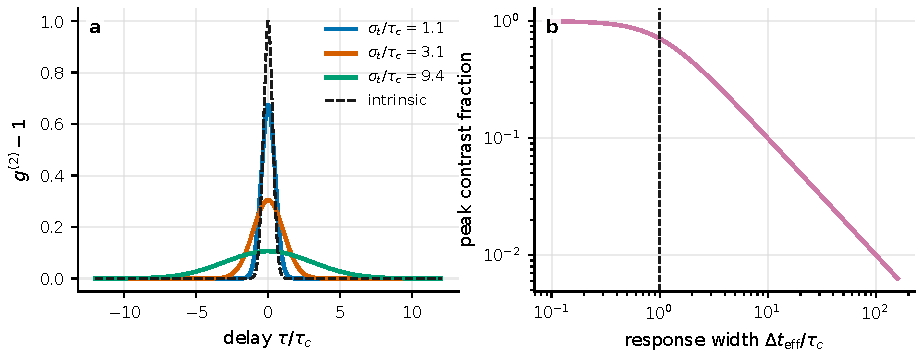
\includegraphics[width=0.95\linewidth]{figures/generated/chapter_04/ch04_response_convolution.pdf}
\caption{A finite time response broadens and lowers the narrow thermal-light bunching peak. Left: the dashed curve is the intrinsic picosecond-scale peak, and the solid curves are the observed peaks after convolution with different response widths; right: when \(\Delta t_{\rm eff}\gg\tau_c\), the zero-delay peak height falls approximately as \(\tau_c/\Delta t_{\rm eff}\): the area is preserved, but the peak height is diluted.}
\label{fig:e08-response}
\end{figure}

\textbf{Plugging in a real yardstick: Guerin's stellar bunching experiment.}\ Guerin et al.\ used a 1-meter telescope, a multimode fiber, a beam splitter, two avalanche photodiodes (APDs), and a delay histogram to measure the thermal-light bunching of a star \citep{2017MNRAS.472.4126G}. Their parameters make an excellent order-of-magnitude exercise: central wavelength about \(7800\,\text{\AA}\), narrowest filter bandwidth \(10\,\text{\AA}\). First compute the coherence time (as in Eq.~\eqref{eq:e08-tauc}): \(\Delta\nu\simeq c\Delta\lambda/\lambda^2\approx5\times10^{11}\,{\rm Hz}\), so \(\tau_c\simeq2\,{\rm ps}\). And the relative response peak width of the two detectors is about \(\Delta t_{\rm eff}\approx700\,{\rm ps}\) (the time jitter of a single APD is about 500 ps). For ideal thermal light \(C_{\rm true}=1\), the temporal dilution alone gives \(\tau_c/\Delta t_{\rm eff}\approx2/700\approx3\times10^{-3}\). This is already the dominant factor in the peak height; beyond it, one must multiply by an \(\mathcal O(1)\) shape/mode coefficient: after the Lorentzian intrinsic peak is convolved with a near-Gaussian response, the zero-delay peak height carries about a \(0.7\) peak-shape discount relative to the crude estimate "area divided by response width," together with residual polarization/mode and background dilution, which push the expected peak height down to

\[
  C_{\rm obs}\approx(2\text{--}3)\times10^{-3}\quad(\text{order-of-magnitude estimate}),
\]

which compares well, to order of magnitude, with the laboratory thermal-source measurement of \((2.01\pm0.09)\times10^{-3}\) and with the peaks of about \(1.8\)--\(2.0\times10^{-3}\) given by three bright stars. The conclusion in one sentence: what pops out directly on a telescope's correlation plot is never the textbook \(g^{(2)}(0)=2\), but an excess of \(1+10^{-3}\), \(1+10^{-6}\), or even smaller. Seeing this small decimal at all relies on the accumulation of a vast number of event pairs.

\paragraph{The Delay Histogram: Turning the Event List into a Correlation Function}
\label{sec:e08-histogram}

So how, concretely, is \(g^{(2)}\) estimated from the event list? The answer is the \textbf{delay histogram}. Take two channels \(A,B\), compute the time difference \(t_{B,j}-t_{A,i}\) of every event pair, and accumulate it into a delay bin of width \(\delta\tau\):

\begin{equation}
  H_{AB}(\tau_m)=\sum_{i\in A}\sum_{j\in B}
  \mathbf{1}\!\left(\tau_m-\tfrac{\delta\tau}{2}\le t_{B,j}-t_{A,i}<\tau_m+\tfrac{\delta\tau}{2}\right),
  \label{eq:e08-histogram}
\end{equation}
\begin{formulaexplain}
\(H_{AB}(\tau_m)\) is the number of event pairs whose delay falls in the \(m\)-th bin (center \(\tau_m\), width \(\delta\tau\)); \(\mathbf 1(\cdot)\) is the indicator function, taking value 1 if it falls within the window and 0 otherwise; the double sum runs over all event pairs of the two channels. It turns the event list directly into the raw counts of the correlation function.
\end{formulaexplain}

To normalize this raw count into a \(g^{(2)}\) that "equals 1 when uncorrelated," divide by the expected number of accidental coincidences. Let the mean count rates of the two channels be \(r_A,r_B\), and the total effective observation time (live time) be \(T\):

\begin{equation}
  \widehat g^{(2)}_{AB}(\tau_m)=\frac{H_{AB}(\tau_m)}{r_A\,r_B\,\delta\tau\,T}.
  \label{eq:e08-estimator}
\end{equation}
\begin{formulaexplain}
\(\widehat g^{(2)}_{AB}\) is the estimator of the second-order correlation; the denominator \(r_Ar_B\,\delta\tau\,T\) is the expected number of accidental coincidences at the same duration, same bin width, and same count rates. Both numerator and denominator are "numbers of pairs," so the ratio is dimensionless and automatically equals 1 when uncorrelated.
\end{formulaexplain}

The rationale of the denominator is straightforward: channel \(A\) has \(r_AT\) events in total, and for each \(A\) event the probability that a \(B\) event falls exactly within its \(\delta\tau\) window is \(r_B\delta\tau\); multiplying the two gives the expected number of accidental coincidences. In practice, analyses often do not use this analytic denominator, but instead construct a reference histogram \(H_{\rm ref}\) from large time offsets, different observing segments, polarization mismatch, or an off-source channel, and then take the ratio: this absorbs systematic effects such as nonuniform TDC bin widths, electronic crosstalk, and slowly varying transparency.

\begin{figure}[tbp]
\centering
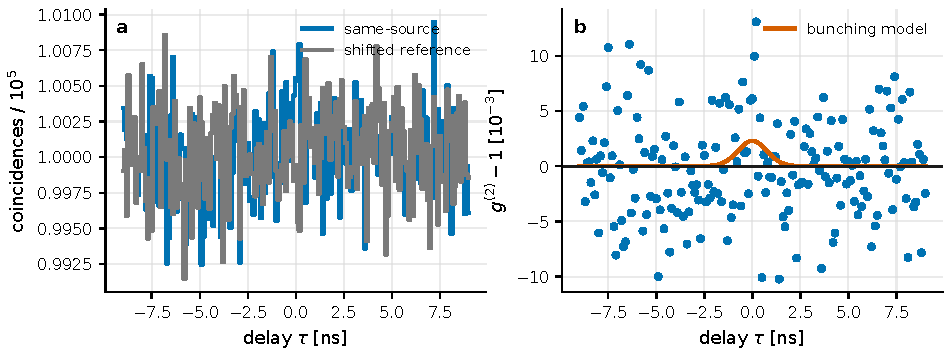
\includegraphics[width=0.95\linewidth]{figures/generated/chapter_04/ch04_delay_histogram_estimator.pdf}
\caption{The structure of the delay-histogram estimator. Left: the histogram of same-source event pairs has, near zero delay, a very small excess of coincidences over the shifted reference histogram; right: normalizing the difference by the number of accidental coincidences gives \(g^{(2)}-1\), with a peak of only the \(10^{-3}\) order. Real observations must further add corrections for dead time, background, and the response function.}
\label{fig:e08-delay-hist}
\end{figure}

\paragraph{Statistical Error: Everything Rests on Counting Enough Event Pairs}
\label{sec:e08-shotnoise}

Where does the precision of the estimator come from? Mainly from the shot noise of the accidental-coincidence pair count. If a given delay bin contains \(N_{\rm pair}\) accidental coincidences, it is Poisson-fluctuating (Chapter \ref{chap:e03}), with standard deviation \(\sqrt{N_{\rm pair}}\), so the relative error is

\begin{equation}
  \sigma\!\left[\widehat g^{(2)}(\tau)\right]\sim\frac{1}{\sqrt{N_{\rm pair}}}.
  \label{eq:e08-shotnoise}
\end{equation}
\begin{formulaexplain}
\(\sigma[\widehat g^{(2)}]\) is the statistical error of the correlation estimator; \(N_{\rm pair}=r_Ar_B\,\delta\tau\,T\) is the number of accidental coincidences in that bin. To push the error below a signal of \(10^{-3}\), one must accumulate an enormous number of event pairs.
\end{formulaexplain}

Let us plug in a set of numbers to feel the difficulty. Take two channels with \(r=10^{6}\,{\rm s^{-1}}\), \(\delta\tau=100\,{\rm ps}=10^{-10}\,{\rm s}\), and \(T=1\,{\rm hr}=3600\,{\rm s}\):
\[
  N_{\rm pair}=r_Ar_B\,\delta\tau\,T
  =(10^6)(10^6)(10^{-10})(3600)
  =3.6\times10^{5},
\]
so the single-bin statistical error is \(\sigma\sim1/\sqrt{3.6\times10^5}\approx1.7\times10^{-3}\). This is almost the same order as Guerin's signal of \(2\times10^{-3}\); that is, one hour and a single delay bin are still far from enough, barely \(1\sigma\). To push the error down to \(10^{-4}\) requires \(N_{\rm pair}\sim10^{8}\), i.e.\ accumulating the pair count from \(3.6\times10^5\) by about \(300\) times more (\(10^8/3.6\times10^5\approx278\)). Note that this factor of 300 scales differently along the two routes: \(N_{\rm pair}\propto T\) is linear in exposure, so the exposure time must be lengthened by about \(300\) times; whereas \(N_{\rm pair}\propto r_Ar_B\) is quadratic in count rate, so raising each channel's count rate by about \(\sqrt{300}\approx17\) times suffices (the third "Questions to Ponder" of this chapter tests exactly this \(r^2\) scaling). Of course one may combine the two, or jointly fit the several bins spanned by the bunching peak (the peak is more than one bin wide, and can be used jointly). This also reminds us of a ceiling: when the systematic correlation (TDC crosstalk, residual background normalization) sits at the \(10^{-3}\) level, adding more exposure cannot substitute for correcting these systematic terms. Modern VERITAS and MAGIC intensity interferometry extends exactly this idea to spatial scales, using offline correlation, GPU/FPGA correlators, and multi-baseline averaging \citep{2020NatAs...4.1164A,2024MNRAS.529.4387A}.

\section{Looking Ahead: Third-Order Correlation and Closure Phase}
\label{sec:e08-g3}

Second-order correlation invokes only photon \emph{pairs}. If we keep three telescopes (or three channels) at once, we can define the third-order intensity correlation:

\begin{equation}
  g^{(3)}_{123}=\frac{\big\langle I_1 I_2 I_3\big\rangle}
  {\big\langle I_1\big\rangle\big\langle I_2\big\rangle\big\langle I_3\big\rangle}.
  \label{eq:e08-g3}
\end{equation}
\begin{formulaexplain}
\(g^{(3)}_{123}\) is the three-channel normalized intensity correlation; \(I_1,I_2,I_3\) are the intensities of the three telescopes; the denominator is the random triple-coincidence baseline. It generalizes the statistical object from "photon pairs" to "photon triplets."
\end{formulaexplain}

For Gaussian chaotic light, one again uses the Gaussian moment theorem to split the sixth-order moment (this time three unstarred and three starred fields paired two by two, with a total of \(3!=6\) legal "starred-with-unstarred" pairings: three of them pair \(I_i\) in place into modulus-squared terms of the \(|\gamma|^2\) type, while a conjugate pair of cyclic pairings combines into the closure term). The result, beyond the modulus-squared terms of the three baselines, contains one extra \emph{triangle closure} term:

\begin{equation}
  g^{(3)}_{123}=1+|\gamma_{12}|^2+|\gamma_{23}|^2+|\gamma_{31}|^2
  +2\,{\rm Re}\!\big(\gamma_{12}\,\gamma_{23}\,\gamma_{31}\big),
  \label{eq:e08-g3-closure}
\end{equation}
\begin{formulaexplain}
\(\gamma_{ij}\) is the first-order degree of coherence (a complex number) between channels \(i,j\); the three modulus-squared terms come from the three baselines; the final term \({\rm Re}(\gamma_{12}\gamma_{23}\gamma_{31})\) is the \textbf{closure phase} term, obtained by adding the phases of the three baselines. It is the entry point by which third-order intensity interferometry reaches phase combinations.
\end{formulaexplain}

The key lies in the final term: in \(\gamma_{12}\gamma_{23}\gamma_{31}\) the phases of the three complex degrees of coherence add up, forming exactly a \emph{closed triangle}. Second-order intensity interferometry gives only \(|\gamma|^2\), throwing the phase away entirely; but this closure phase in the third-order term is measurable. This points directly to the imaging phase problem of Chapter \ref{chap:e11}: intensity interferometry innately loses phase, and the closure phase (along with higher-order correlations) is one route to recovering phase combinations. The price is much greater noise: photon triplets are far rarer than photon pairs, and more sensitive to systematic errors. Gamo's early theory and the imaging simulations of Nuñez et al.\ both treat higher-order correlation as an important extension of intensity-interferometric imaging \citep{1966JOSA...56..441G,2012MNRAS.419..172N}.

\begin{figure}[tbp]
\centering
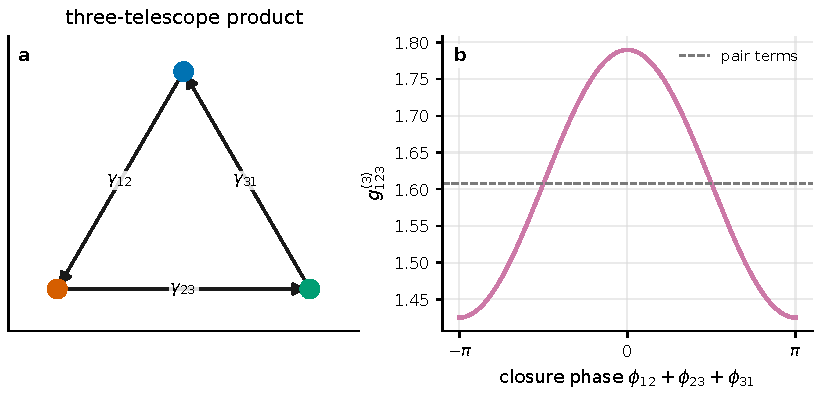
\includegraphics[width=0.92\linewidth]{figures/generated/chapter_04/ch04_g3_closure_phase.pdf}
\caption{The origin of the closure-phase term in the third-order intensity correlation. Left: three telescopes form the closed product \(\gamma_{12}\gamma_{23}\gamma_{31}\); right: at fixed \(|\gamma_{ij}|\), \(g^{(3)}\) varies as the cosine of the closure phase. Second-order intensity interferometry gives only \(|\gamma|^2\); only the third-order term begins to be sensitive to phase combinations.}
\label{fig:e08-g3}
\end{figure}

\section{A Door: Trading the Time Delay for a Spatial Baseline}
\label{sec:e08-gateway}

From start to finish this chapter has spoken of the "time delay \(\tau\)," the echo of the same beam of light across a delay \(\tau\). The final step is to replace the \(\tau\) of this language with a \emph{spatial baseline} \(\bm B\), and a door opens onto Chapter \ref{chap:e10}.

Imagine two telescopes separated by \(\bm B\) staring at the same star at once, each recording intensity fluctuations. Replace the two "instants" of \(g^{(1)}\) with two "positions," and it no longer measures "how much phase the field remembers across \(\tau\)," but "how coherent the field is at two points separated by \(\bm B\)." And the van Cittert--Zernike theorem (to be proved in Chapter \ref{chap:e10}) will tell us: this spatial version of \(g^{(1)}(\bm B)\) is exactly the \textbf{complex visibility} of the sky brightness distribution: it is a Fourier component of the source's angular structure. So the Siegert relation carries over unchanged:

\[
  g^{(2)}(\bm B)-1=\zeta\,\big|g^{(1)}(\bm B)\big|^2
  =\zeta\,\big|V(\bm B)\big|^2 ,
\]

and the \emph{degree of synchrony} of the intensity fluctuations of the two telescopes directly yields the squared modulus of the complex visibility, \(|V(\bm B)|^2\). This is the whole magic of HBT intensity interferometry: without combining the electric fields of the two telescopes through a vacuum pipe as amplitude interferometry does (an almost punishing demand on optical-path stability), one measures the squared visibility simply by comparing, after the fact, the intensity fluctuations recorded separately at the two sites, and thereby infers the star's angular diameter. The prerequisite for validity remains the two conditions this chapter has stressed repeatedly: the source light is approximately Gaussian chaotic light, and the instrument normalization has not mixed the background, mode number, and time response into \(\zeta\).

Carrying this door with us, we can step into Chapter \ref{chap:e10}: upgrading "temporal correlation" into "spatial correlation," upgrading "coherence time" into "visibility curve," and finally, in Chapter \ref{chap:e11}, inferring the image of a celestial object from the visibility.

\section{Chapter Summary}
\label{sec:e08-summary}

\begin{itemize}
  \item \textbf{Two orders of coherence, two plain questions.} First order \(g^{(1)}(\tau)\) (Eq.~\eqref{eq:e08-g1}) measures the phase memory of the field: \(|g^{(1)}|\to1\) coherent, \(\to0\) amnesic, and its decay width is the coherence time \(\tau_c\simeq1/\Delta\nu\) (780\,nm/1\,nm gives \(\tau_c\approx2\,{\rm ps}\)). Second order \(g^{(2)}(\tau)\) (Eq.~\eqref{eq:e08-g2-field}) measures the tendency of photons to arrive in pairs.
  \item \textbf{Three statistics, three peaks.} Poisson (coherent state) \(g^{(2)}=1\); thermal-light bunching \(g^{(2)}(0)=2\); \(g^{(2)}(0)<1\) antibunching, a nonclassical signature. The classical form \(g^{(2)}=\langle II\rangle/\langle I\rangle^2\) is handy, but beware whether \(I\) has already been convolved by the response.
  \item \textbf{The Siegert relation is the bridge of this chapter.} \(g^{(2)}(\tau)=1+\zeta|g^{(1)}(\tau)|^2\) (Eq.~\eqref{eq:e08-siegert}), coming from the fourth-order-moment split of Gaussian chaotic light (the Gaussian-moment/Wick theorem): \(\langle II\rangle=\langle I\rangle^2+|G^{(1)}|^2\). It lets the intensity correlation directly read off the squared field coherence. The spectral shape sets the peak shape: rectangular sinc\(^2\), Lorentzian exponential, Gaussian Gaussian. \(\zeta\) collects only mode number, polarization, and background (the finite time response is handled separately by convolution and is not included in \(\zeta\)). \emph{It does not hold for coherent states.}
  \item \textbf{Dilution in the telescope.} The finite-response convolution preserves area but not peak height, \(C_{\rm obs}\simeq C_{\rm true}(\tau_c/\Delta t_{\rm eff})(1/M)f_Af_B\) (Eq.~\eqref{eq:e08-contrast}). Guerin's experiment: \(7800\,\text{\AA}\), \(10\,\text{\AA}\), \(\tau_c\approx2\,{\rm ps}\), response \(\approx700\,{\rm ps}\), observed peak only \(C_{\rm obs}\approx2\times10^{-3}\).
  \item \textbf{Estimator and noise.} The delay histogram \(\widehat g^{(2)}=H_{AB}/(r_Ar_B\,\delta\tau\,T)\) (Eq.~\eqref{eq:e08-estimator}), with error \(\sigma\sim N_{\rm pair}^{-1/2}\) (Eq.~\eqref{eq:e08-shotnoise}): everything rests on counting enough event pairs.
  \item \textbf{Two doors.} The closure-phase term of the third-order \(g^{(3)}\) leads to the imaging phase problem of Chapter \ref{chap:e11}; replacing \(\tau\) with the baseline \(\bm B\) turns \(g^{(1)}\) into the complex visibility \(V(\bm B)\), leading to the spatial intensity interferometry of Chapter \ref{chap:e10}.
\end{itemize}

\medskip
\noindent\textbf{Questions to Ponder.}
\begin{enumerate}
  \item If the filter bandwidth is broadened from \(10\,\text{\AA}\) to \(100\,\text{\AA}\), how does the coherence time \(\tau_c\) change? With the response \(\Delta t_{\rm eff}\approx700\,{\rm ps}\) unchanged, will the observed peak height \(C_{\rm obs}\) rise or fall, and by roughly what factor?
  \item Someone measures a source whose \(g^{(1)}\) remains close to 1 over very long delays, yet finds \(g^{(2)}\equiv1\). Is this more likely thermal light or a laser? Why does it not violate the Siegert relation?
  \item If the count rates of the two channels are each raised by 10 times and the exposure time lengthened by 4 times, by what factor does the single-bin accidental-coincidence number \(N_{\rm pair}\) change? And by what factor does the corresponding statistical error \(\sigma[\widehat g^{(2)}]\) change?
\end{enumerate}
